\documentclass[12pt]{article}

\usepackage{sbc-template}
\usepackage{graphicx,url}
\usepackage[utf8]{inputenc}
\usepackage[T1]{fontenc}
\usepackage[brazil]{babel}
\usepackage{booktabs}
\usepackage{amsmath}
\usepackage[hidelinks]{hyperref}

\sloppy
\setlength{\textfloatsep}{6pt plus 2pt minus 2pt}
\setlength{\floatsep}{6pt plus 2pt minus 2pt}
\setlength{\intextsep}{6pt plus 2pt minus 2pt}
\setlength{\abovecaptionskip}{3pt}

% >>> LINK DO REPOSITÓRIO: troque o espaço em branco abaixo pelo link, por exemplo:
%     \newcommand{\repositorio}{\url{https://github.com/usuario/trabalho_series_temporais}}
\newcommand{\repositorio}{\underline{\hspace{8cm}}}

\title{Reconhecimento Antecipado de Sinais Isolados de Libras\\
como Classificação de Séries Temporais Multivariadas}

\author{Magnus Victor Lopes Felinto de Oliveira\inst{1}}

\address{Programa de Pós-Graduação em Ciência da Computação (PPgCC UERN/UFERSA)\\
  Tópicos Especiais em ESSC II -- IA Aplicada a Séries Temporais
  \email{magnus.oliveira89457@alunos.ufersa.edu.br}
}

\begin{document}
\renewcommand{\refname}{Referências}
\maketitle

\begin{resumo}
Vídeos do MINDS-Libras (20 palavras, 12 sinalizantes) viram séries multivariadas de \textit{keypoints} (32 instantes $\times$ 321 canais), avaliadas em sinalizantes nunca vistos. Comparamos baselines, árvores sobre \textit{lags}, redes convolucionais, recorrentes, híbridas e Transformers, com ablação de pré-processamento e análise do horizonte (classificação antecipada). A CNN-1D sobre a 1ª diferença obteve F1 macro de 92,6\%; suavização, aumento de dados e redes mais profundas não ajudaram; 50\% do sinal bastam para $\sim$90\% de F1.
\end{resumo}

\begin{abstract}
MINDS-Libras videos (20 words, 12 signers) become multivariate keypoint series (32 steps $\times$ 321 channels), evaluated on unseen signers. We compare baselines, trees on lags, convolutional, recurrent, hybrid and Transformer networks, with a preprocessing ablation and an early-classification horizon analysis. A 1D CNN on first differences reached 92.6\% macro F1; smoothing, augmentation and deeper networks did not help; 50\% of the signal suffices for $\sim$90\% F1.
\end{abstract}

\section{Introdução}

Um sinal da Língua Brasileira de Sinais (Libras) é um processo físico com seta do tempo: a mão sai do repouso, executa um percurso com configuração, locação e orientação próprias e retorna. A ordem é causal e carrega significado: inverter o tempo produz outro gesto. Por isso tratamos o reconhecimento de sinais isolados como \textbf{classificação} (20 classes) \textbf{de séries temporais multivariadas}: cada vídeo vira uma série de posições do corpo e das mãos, sem variáveis exógenas. O desafio é a \textbf{mudança de distribuição entre pessoas}.

Como a tarefa não é de previsão, o \textbf{horizonte} foi adaptado (com aval do professor) para \textbf{classificação antecipada}: o modelo recebe apenas a fração inicial $h \in \{12{,}5\%, \dots, 100\%\}$ do sinal, o que equivale a reduzir o tempo de exposição. As questões de pesquisa são: \textbf{(Q1)}~qual família de modelos generaliza melhor para sinalizantes novos? \textbf{(Q2)}~o pré-processamento (decomposição, frequência, diferenciação) melhora o resultado? \textbf{(Q3)}~quão cedo é possível reconhecer o sinal?

\section{Metodologia}

\textbf{Dados.} O MINDS-Libras \cite{rezende2021} tem vídeos a $\sim$30~fps (3 a 7~s) de 20 palavras por 12 sinalizantes (1.158 vídeos processados). O MediaPipe Holistic extrai 33 pontos do corpo e 21 de cada mão em 32 quadros uniformes. Falhas curtas da mão ($\le$4 quadros) são interpoladas, o repouso inicial e final é cortado e o trecho ativo é reamostrado para \textbf{32 instantes}. As coordenadas são normalizadas pelo corpo (centro e largura dos ombros), a mão dominante é espelhada para uma coluna fixa e a forma de cada mão é expressa em relação ao próprio pulso, totalizando \textbf{321 canais} (corpo 75, mãos 2$\times$63, dedos relativos 2$\times$60). ADF e KPSS discordam em nível e na 1ª diferença (baixo poder com 32 pontos) e a ACF/PACF indica dinâmica AR(2) de ida e volta: cada série é um evento transitório, sem sazonalidade, o que descarta a STL.

\textbf{Divisão e protocolo anti-vazamento.} Como os vídeos são independentes, a divisão cronológica é substituída pela divisão por \textbf{sinalizante}: 4 grupos intercalados de 3 pessoas; na rodada $k$, o grupo $k$ é teste, 2 pessoas do grupo seguinte são validação e as 7 restantes, treino ($\sim$670/195/290 vídeos). O \textit{z-score} é ajustado só no treino. Cada configuração roda 4 rodadas $\times$ 3 sementes fixas (12 avaliações), com \textit{early stopping} na validação (paciência 25). Métricas: F1 macro (principal), acurácia e acurácia balanceada (as classes são quase balanceadas); diferenças são testadas com Wilcoxon pareado (mesma rodada e semente).

\textbf{Pré-processamento (ablação).} (i) \textbf{Decomposição} por média móvel centrada ($k$=3), mantendo a tendência; (ii) \textbf{filtro passa-baixa por FFT} (10 primeiras frequências); (iii) ambos; (iv) \textbf{1ª diferença} $\Delta x_t = x_t - x_{t-1}$ (velocidades); (v) $X$+$\Delta$. Os parâmetros de (i) e (ii) foram escolhidos na validação.

\textbf{Arquiteturas.} Baselines: classe majoritária e 1-NN+DTW (banda de Sakoe-Chiba na validação). (A)~Árvore de Decisão, Random Forest e XGBoost sobre a janela de 32 \textit{lags} achatada. (B)~CNN-1D (3 convoluções 64/128/128, \textit{batch norm}, média global) e WaveNet \cite{oord2016} (convoluções causais com portas, dilatações 1--16). (C)~SimpleRNN, LSTM \cite{hochreiter1997} e GRU \cite{cho2014} (2 camadas de 128). (D)~Híbrida Conv1D+\textit{max-pooling}+GRU. Todas em TensorFlow/Keras (Adam, ruído gaussiano na entrada, \textit{dropout}), recalibradas na validação. No horizonte, comparamos o modelo do sinal completo (\textit{sem adaptação}), um modelo por horizonte (estratégia \textit{direta} \cite{bontempi2013}) e um modelo único com prefixos aleatórios; a recursiva não se aplica (não há valores futuros a prever).

\section{Resultados e Discussão}

A Tabela~\ref{tab:geral} resume todas as arquiteturas; o acaso fica em 5\% e o 1-NN+DTW em 61,5\%. \textbf{Q1.} As convolucionais generalizam melhor; a CNN-1D é o melhor modelo sobre o sinal bruto, seguida da híbrida e do Random Forest. As recorrentes decoram os sinalizantes de treino (Figura~\ref{fig:curvas}): a perda de treino vai a zero e a de validação estaciona alta, e a SimpleRNN fracassa mesmo calibrada. A calibração não altera a ordem. O mesmo modelo varia até $\sim$0,8 ponto entre execuções (não determinismo da GPU); diferenças menores não são interpretadas.

\begin{table}[!t]
\centering\footnotesize
\caption{Teste com sinalizantes nunca vistos (média $\pm$ desvio, 4 rodadas $\times$ 3 sementes). Calib.: hiperparâmetros escolhidos na validação.}\label{tab:geral}
\begin{tabular}{llccc}
\toprule
Grupo & Modelo & F1 (\%) & Acc. (\%) & F1 calib. (\%) \\
\midrule
Baselines & Classe majoritária & 0{,}5 & 5{,}2 & -- \\
 & 1-NN + DTW & 61{,}5 $\pm$ 6{,}0 & 62{,}1 & -- \\
A -- Tabular (lags) & Árvore de Decisão & 71{,}2 $\pm$ 2{,}7 & 72{,}2 & -- \\
 & Random Forest & 89{,}0 $\pm$ 3{,}6 & 90{,}2 & -- \\
 & XGBoost & 87{,}6 $\pm$ 3{,}7 & 88{,}5 & -- \\
B -- Convolucional & CNN-1D & 91{,}3 $\pm$ 2{,}5 & 92{,}0 & 91{,}1 $\pm$ 2{,}2 \\
 & WaveNet & 87{,}9 $\pm$ 2{,}3 & 88{,}7 & 87{,}9 $\pm$ 2{,}5 \\
C -- Recorrente & SimpleRNN & 46{,}4 $\pm$ 10{,}2 & 48{,}1 & 53{,}9 $\pm$ 4{,}6 \\
 & LSTM & 78{,}2 $\pm$ 3{,}1 & 79{,}6 & 78{,}0 $\pm$ 3{,}8 \\
 & GRU & 84{,}3 $\pm$ 3{,}7 & 85{,}2 & 83{,}9 $\pm$ 3{,}8 \\
D -- Híbrido & Conv1D + GRU & 89{,}0 $\pm$ 1{,}4 & 89{,}6 & 88{,}6 $\pm$ 1{,}7 \\
\textbf{Melhor combinação} & \textbf{CNN-1D + $\Delta$} & \textbf{92{,}6 $\pm$ 3{,}6} & \textbf{93{,}5} & -- \\
\midrule
E -- Bônus I & Transformer multicanal & 90{,}4 $\pm$ 1{,}9 & 91{,}2 & -- \\
 & PatchTST & 79{,}0 $\pm$ 8{,}3 & 80{,}3 & -- \\
E -- Bônus II & FCN & 90{,}8 $\pm$ 2{,}5 & 91{,}5 & -- \\
 & ResNet & 84{,}7 $\pm$ 5{,}9 & 85{,}7 & -- \\
 & InceptionTime & 87{,}3 $\pm$ 3{,}2 & 88{,}2 & -- \\
\bottomrule
\end{tabular}
\end{table}

\begin{figure}[!t]
\centering
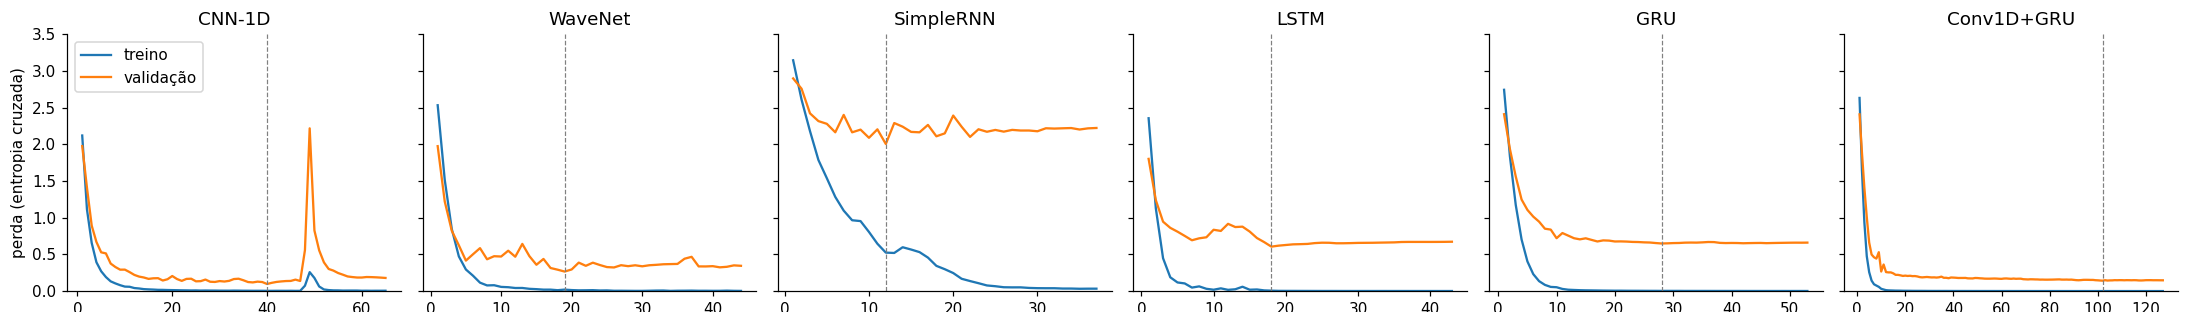
\includegraphics[width=\textwidth]{fig/curvas_perda.png}
\caption{Curvas de aprendizado (entropia cruzada; rodada 0, semente 0). Tracejado: época restaurada pelo \textit{early stopping}.}\label{fig:curvas}
\end{figure}

\textbf{Q2 (ablação, Tabela~\ref{tab:ablacao}).} A suavização não ajuda nenhum modelo e piora a GRU: o ruído do MediaPipe não é o gargalo, e a média móvel apaga transições rápidas da mão. A \textbf{1ª diferença} é a única técnica com ganho, e só na CNN-1D (+2,2, $p$=0,034), levando ao melhor resultado do trabalho (92,6\%). Ela remove o deslocamento próprio de cada pessoa, principal fonte de erro com sinalizantes novos, mas apaga a locação para os modelos que não a reconstroem (RF $-$12,5; GRU $-$13,2); $X$+$\Delta$ os recupera.

\begin{table}[!t]
\centering\footnotesize
\caption{Ablação: variação do F1 (pontos) de cada técnica em relação ao sinal bruto (Wilcoxon pareado, 12 pares: * $p<0{,}05$; ** $p<0{,}01$; *** $p<0{,}001$). $\Delta$ e $X$+$\Delta$ vêm de uma reexecução, comparada ao próprio bruto (CNN-1D: 90,5).}\label{tab:ablacao}
\begin{tabular}{lcccccc}
\toprule
Modelo & Bruto & MM ($k$=3) & FFT & MM+FFT & $\Delta$ & $X$+$\Delta$ \\
\midrule
Random Forest & 89{,}0 & +0{,}4 & $-$0{,}1 & +0{,}1 & $-$12{,}5*** & +0{,}2 \\
CNN-1D & 91{,}2 & $-$0{,}2 & $-$0{,}8 & +0{,}2 & \textbf{+2{,}2*} & +1{,}5** \\
GRU & 83{,}8 & $-$5{,}5** & $-$0{,}5 & $-$7{,}0*** & $-$13{,}2*** & $-$1{,}4 \\
Conv1D+GRU & 88{,}4 & $-$0{,}6 & $-$0{,}1 & $-$1{,}9 & $-$15{,}6*** & $-$0{,}9 \\
\bottomrule
\end{tabular}
\end{table}

\textbf{Q3 (horizonte, Figura~\ref{fig:horizonte}).} Com 50\% do trecho ativo, a CNN-1D já atinge 90,3\% de F1, praticamente o mesmo que com o sinal inteiro (91,2\%). Abaixo disso a queda é rápida, e a estratégia direta só compensa nos horizontes curtos (25\%: 69,6\% contra 58,0\% sem adaptação). A GRU direta é melhor com 75\% do que com 100\% do sinal (89,4\% contra 83,8\%): como decide pelo último estado, a fase de retração a atrapalha. O mapa de ativação de classe (CAM) \cite{wang2017} da CNN-1D explica o resultado: a evidência se concentra no núcleo do gesto (instantes $\sim$8 a 24) e quase não está na preparação e na retração.

\begin{figure}[!t]
\centering
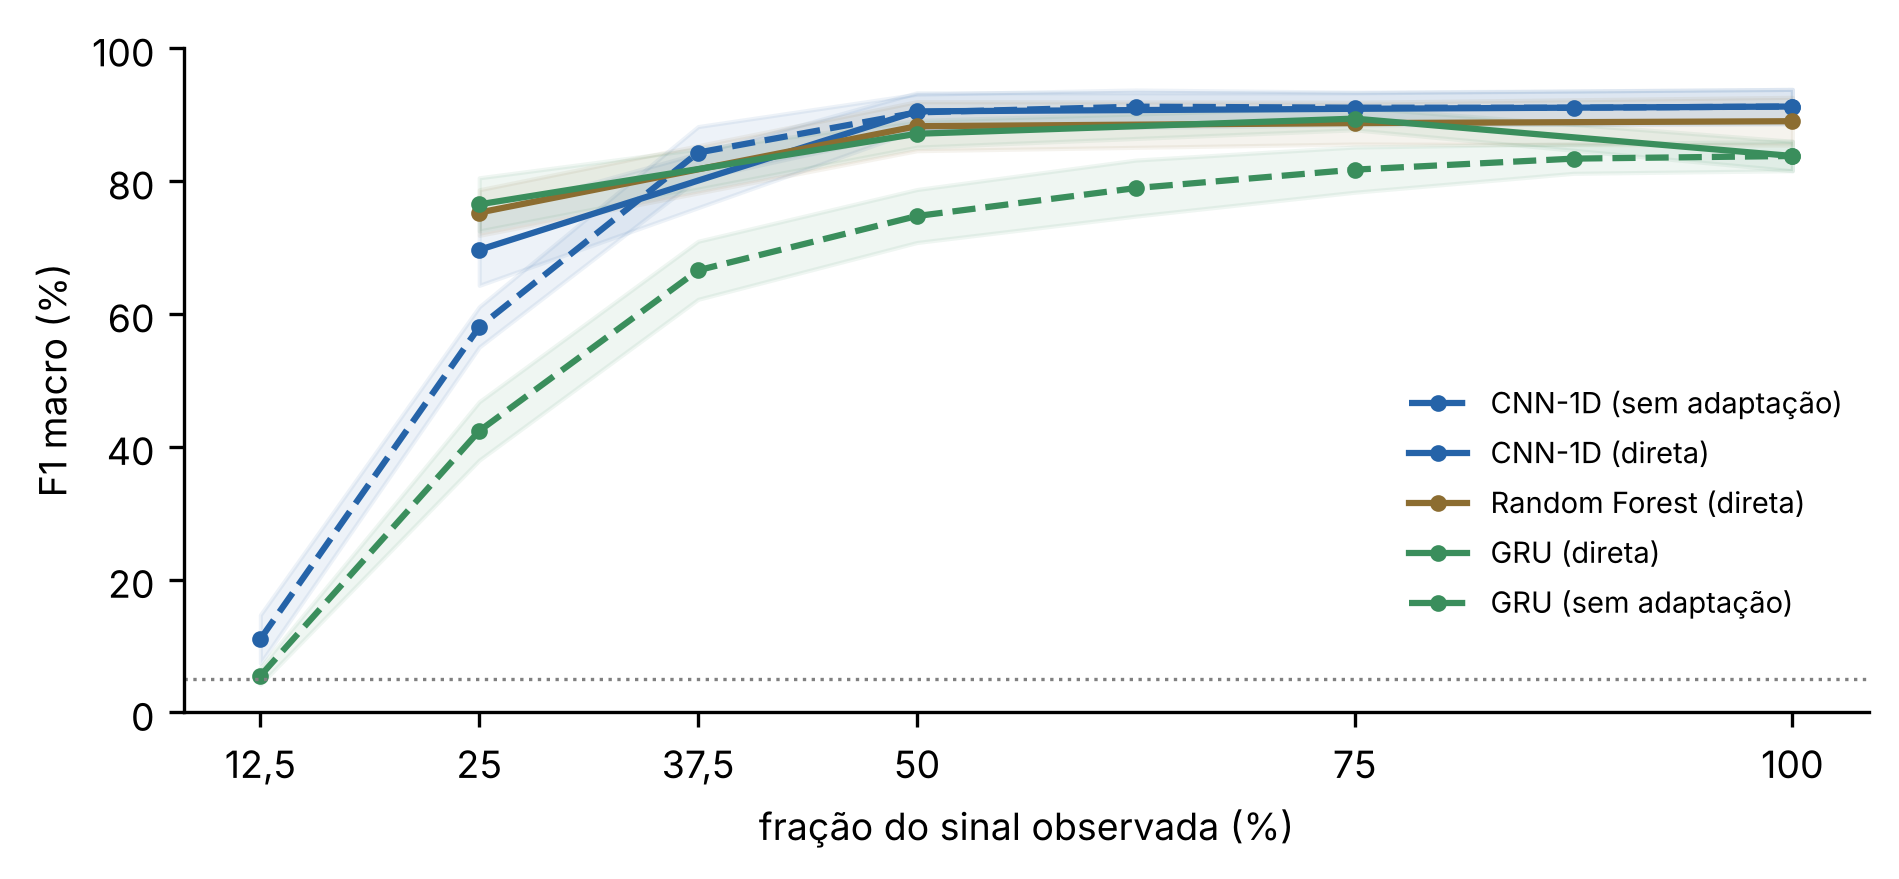
\includegraphics[height=3.6cm]{fig/08_horizonte.png}\hspace{4mm}
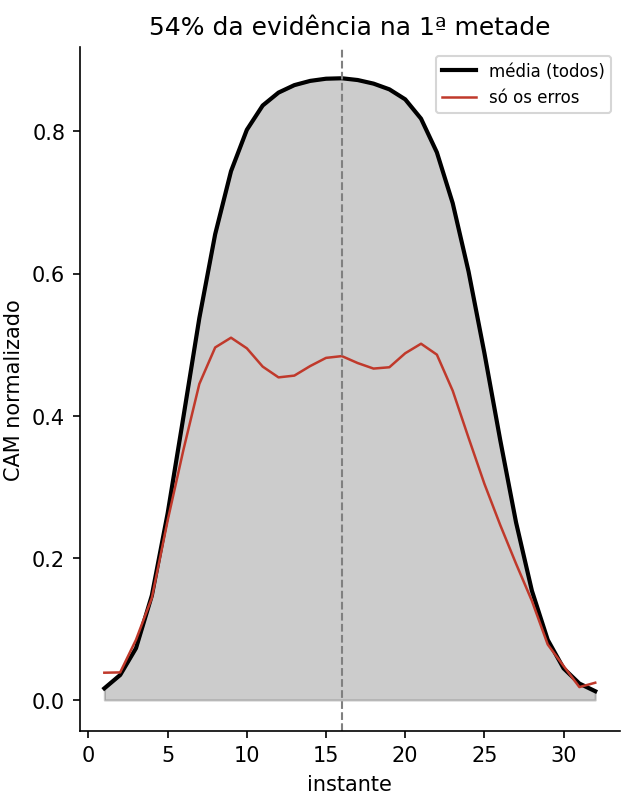
\includegraphics[height=3.6cm]{fig/cam_media.png}
\caption{Esquerda: F1 macro por fração observada do sinal (faixas: $\pm$1 desvio). Direita: CAM médio da CNN-1D na classe verdadeira, para todos os vídeos e só para os erros.}\label{fig:horizonte}
\end{figure}

\textbf{Bônus.} Avaliamos, do survey de DTSF \cite{kong2025}, o \textbf{PatchTST} \cite{nie2023} (patches de 4 instantes, canais independentes) e um Transformer de patches multicanal; do survey de classificação \cite{foumani2024}, FCN, ResNet \cite{wang2017}, InceptionTime \cite{fawaz2020} e aumento de dados \cite{um2017}. Mais complexidade não compensou. O PatchTST perde 11,8 pontos ($p<$0,001) com $\sim$10$\times$ o tempo de treino: a independência de canais ignora a relação entre a mão e a locação no corpo. O Transformer multicanal e a FCN empatam com a CNN-1D; ResNet e InceptionTime perdem 5,8 e 3,2 pontos ($p$=0,009), decorando o treino mais cedo. O conjunto de 3 sementes ajuda (+1,1), mas triplica o custo. Deformação do tempo, escala e deformação de amplitude não melhoram a CNN-1D+$\Delta$ ($-$0,2 a $-$1,4, n.s.), porque a reamostragem e a normalização pelos ombros já removem duração e escala. Por gradiente$\times$entrada, os \textbf{dedos da mão dominante} são o grupo mais informativo (1,6$\times$ a média por canal), coerente com a configuração de mão como parâmetro fonológico.

\section{Conclusão}

Uma CNN-1D simples sobre a 1ª diferença reconheceu palavras de pessoas nunca vistas com F1 macro de 92,6\%, superando árvores, recorrentes, Transformers e CNNs mais profundas; a suavização não ajuda e metade do sinal basta para $\sim$90\% de F1. O limite é a variação entre sinalizantes, não a capacidade do modelo. \textbf{Limitações:} a base é pequena (20 palavras, 12 pessoas); o recorte do trecho ativo usa o vídeo inteiro, então a classificação antecipada assume que o início do sinal é conhecido; e há variação de $\sim$0,8 ponto entre execuções. \textbf{Trabalhos futuros:} redes de grafos espaço-temporais sobre o esqueleto, pré-treino auto-supervisionado em bases maiores e detecção do início do sinal em fluxo contínuo. \textbf{Código, notebooks com sementes fixas e resultados:} \repositorio.

\begin{thebibliography}{99}\footnotesize\setlength{\itemsep}{0pt}

\bibitem{bontempi2013}
Bontempi, G., Ben Taieb, S. e Le Borgne, Y.-A. (2013). Machine learning strategies for time series forecasting. In \textit{Business Intelligence (eBISS 2012)}, LNBIP 138, p. 62--77. Springer.

\bibitem{cho2014}
Cho, K. et al. (2014). Learning phrase representations using RNN encoder-decoder for statistical machine translation. In \textit{Proc. EMNLP}, p. 1724--1734.

\bibitem{fawaz2020}
Fawaz, H. I. et al. (2020). InceptionTime: finding AlexNet for time series classification. \textit{Data Mining and Knowledge Discovery}, 34(6):1936--1962.

\bibitem{foumani2024}
Foumani, N. M. et al. (2024). Deep learning for time series classification and extrinsic regression: a current survey. \textit{ACM Computing Surveys}, 56(9):1--45.

\bibitem{hochreiter1997}
Hochreiter, S. e Schmidhuber, J. (1997). Long short-term memory. \textit{Neural Computation}, 9(8):1735--1780.

\bibitem{kong2025}
Kong, X. et al. (2025). Deep learning for time series forecasting: a survey. \textit{International Journal of Machine Learning and Cybernetics}, 16(7):5079--5112.

\bibitem{nie2023}
Nie, Y. et al. (2023). A time series is worth 64 words: long-term forecasting with Transformers. In \textit{Proc. ICLR}.

\bibitem{oord2016}
van den Oord, A. et al. (2016). WaveNet: a generative model for raw audio. \textit{arXiv:1609.03499}.

\bibitem{rezende2021}
Rezende, T. M. et al. (2021). Development and validation of a Brazilian sign language database for human gesture recognition. \textit{Neural Computing and Applications}, 33:10449--10467.

\bibitem{um2017}
Um, T. T. et al. (2017). Data augmentation of wearable sensor data for Parkinson's disease monitoring using convolutional neural networks. In \textit{Proc. ACM ICMI}, p. 216--220.

\bibitem{wang2017}
Wang, Z., Yan, W. e Oates, T. (2017). Time series classification from scratch with deep neural networks: a strong baseline. In \textit{Proc. IJCNN}, p. 1578--1585.

\end{thebibliography}

\end{document}
